% Ch1Introduction.tex

\chapter[Overview]{Overview}
\label{cha:cha1Introduction}

%=============
\section{Motivation and background}
During the past decades, rapid decreases in frog populations have been spotted from locations around the world, which are regarded as one of the most critical threats to the global biodiversity. Many environment problems are regarded as the reasons for these declines: disease, habitat destruction and modification, exploitation, pollution, pesticide use, introduced species, and ultraviolet-B radiation (UV-B). 
On one hand frog populations are rapidly worldwide declining, and on the other frogs are greatly important to the global ecosystem. 
\begin{enumerate}
\item[(1)] Frogs are integral part of the food web
\item[(2)] Frogs are often used as the environment indicators 
\item[(3)] Frogs are important in medical research that benefits humans 
\end{enumerate}

For those aforementioned reasons, increasing frog populations and optimising the protection policy necessitates monitoring of frogs. Frogs are often much easier to be heard than to be seen (Figure.~\ref{fig:Ch1_frogs}). Also frog vocalizations are often employed for most communication, which offer a possible way to study and evaluate frog populations by detecting species-specific calls \citep{dorcas2009auditory}. Therefore, frogs are often monitored via their vocalisations. Traditional manual monitoring methods require ecologists and volunteers to spend extensive time in the field for  acoustic data collection. Although traditional methods can provide an accurate measure of daytime species and richness, it has a scale limitation in both spatial and temporal domains for this measurement.
To address this limitation, recent advances in acoustic sensors provide a way to automatically survey vocal animals (such as frogs). Deploying acoustic sensors in the field, frog vocalisations can then be automatically collected. Compared with the manual point-counting method, sensors can greatly extend the survey into larger spatial and temporal scales, and generate large volumes of acoustic data that needs to be analysed. Consequently, enabling automatic species identification in acoustic data has become important. However, since the recordings are automatically collected from the field, the audio data tends to be very noisy. Very often the desired signal (frog call) is weak, and there are multiple overlapping signals over the frog call. Furthermore, different frog species tend to call together to make chorus. All those characteristics pose a big challenge to monitor frog vocalisations automatically.

\begin{figure*}[htb!]
\centering
      \begin{subfigure}[b]{0.5\textwidth}
           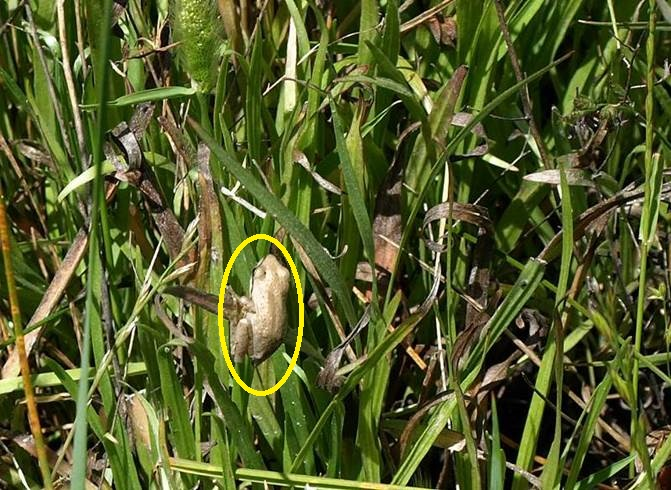
\includegraphics[width=1\textwidth,height=0.75\textwidth]{image/Ch1/unseen_frog_1.jpg}
    \end{subfigure}%
	~~
	      \begin{subfigure}[b]{0.5\textwidth}
           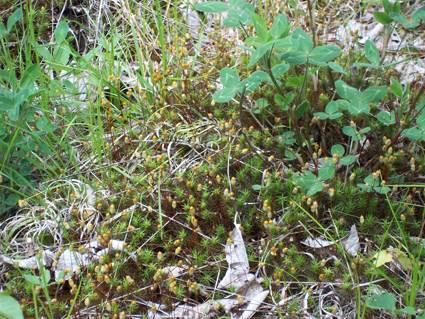
\includegraphics[width=1\textwidth,height=0.75\textwidth]{image/Ch1/unseen_frog_2.jpg}
    \end{subfigure}%
\caption[Photos of frogs]{Photos of frogs to indicate that frogs are difficult to be seen in the field}
\label{fig:Ch1_frogs}       % Give a unique label
\end{figure*}



%===============
\section{Basic concepts} 
In this section, some basic concepts are given to better describe the research problem and questions, aims and objectives, significance and contributions in the following sections.

\subsection{Environmental audio data}
The audio data used in this study is mainly derived from two sources: David Stewart's CD \citep{CD} and recordings collected by James Cook University (JCU) \footnote{All the recordings can be obtained from our group website: https://www.ecosounds.org/}. 
David Stewart's CD is employed for the preliminary testing, and used for the experiments in chapters \ref{cha:cha4EnhancedFeature} and \ref{cha:cha5Wavelet}. 
Recordings collected by JCU are used for chapters \ref{cha:cha6MIML} and \ref{cha:cha7ML}. 
The reasons for using those two datasets are list as follows:
\begin{itemize}
\item  Almost all prior work studied frog recordings with an assumption that only one frog species exists in each individual recording, we first review those previous methods and develop a frog call classification system to outperform the state-of-the-art, where the CD recordings are used for testing. In this thesis, CD recordings are used in chapter \ref{cha:cha4EnhancedFeature} and \ref{cha:cha5Wavelet}.


\item  Compared with the CD recordings, most JCU recordings have multiple simultaneously vocalising frog species, which is accord with the real environment. Chapters \ref{cha:cha6MIML} and \ref{cha:cha7ML} focus on the investigation of JCU recordings, which is the real situation for most environmental recordings. 


\end{itemize}


Compared with audio data collected in the laboratories and quiet places (such as David Stewart’s CD), environmental recordings are normally collected under unconstrained noisy conditions (such as JCU recordings). Consequently, the noise and variability issues need to be considered when coping with environmental audio data. 
For the background noise, there are a wide variety of non-biological noises and a variety of animal sounds in the environmental recordings. These non-biological noises often come from different sources: rain, wind, human activities (e.g. traffic noise). Besides non-biological noises, many competitive animal sounds (e.g. birds when we are interested in frogs) are also recorded in the environmental  recordings. The SNR of CD recordings and JCU recordings are list in 
Table~\ref{tab:wav_spec_cd} and Table~\ref{tab:JCU_para}. The SNR is calculated as follows:

\begin{equation}
SNR=10*log_{10}(\frac{\sum_{i=m}^{m+L}S_{i}^2}{\sum_{j=n}^{n+L}N_{j}^2})
\end{equation}
where $L$ is the length of the signal and noise used for calculating SNR, and set at 6000 samples here, $n$ and $m$ are manual selected start location in the waveform for noise and signal, respectively. 



Since the power of signal and background noise in this study vary from recordings to recordings and calls to calls within the recording, Table~\ref{tab:CI_CD} and Table~\ref{tab:CI_JCU} calculate the confidence intervals of high and low SNR recordings for the power of signal and noise. The calculation of confidence interval is defined as follows:

\begin{equation}
CI=\mu \pm Z*\frac{\sigma}{\sqrt{L}}
\end{equation}
where $\mu$ and $\sigma$ are the mean and standard deviation, respectively, $Z$ is the upper $\frac{(1-C)}{2}$ critical value for the standard normal distribution, $C$ is the confidence level, and set at 0.95.



In the case of variability, it is produced in many aspects: call structure between species, population of one specific species, time and season changes. All those noises and variabilities make it a challenge to develop a robust frog call classification system. 






\subsection{Audio data analysis}
Audio data is usually considered as a mono-dimensional signal. To ease the tasks of understanding, comparison, modification, and resynthesise of signals \citep{rocchesso2003introduction}, audio data analysis is often developed to find the major features representing the time-varying audio data. Many application areas of audio data analysis have been identified: speech processing, mechanical signal processing, bioacoustics analysis, etc. Two most important audio data analysis techniques are Short-time Fourier Transform (STFT) and Linear Predictive Coding (LPC). STFT is a Fourier-related transform, which determines the sinusoidal frequency and phase content of local sections of a signal as it changes over the time \citep{allen1997short}. LPC is mostly used to represent the spectral envelope of an audio data based on the information of a linear predictive model \citep{deng2003speech}. After STFT, the audio data is transformed to its two dimensional representation (spectrogram), which is widely used for most bioacoustics analysis for its flexible implementation and good applicability.
An example of a spectrogram of frog calls derived from a field recording is shown in Figure.~\ref{fig:Ch1_spectrogram}.

\begin{figure}[htb!]
\centering
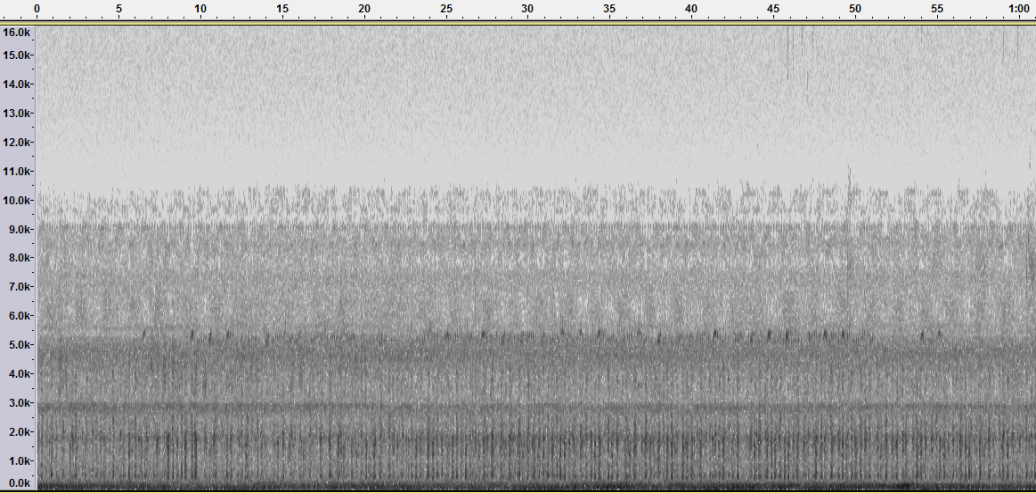
\includegraphics[width=\textwidth]{image/Ch1/spectrogram_example.png}
\caption[An example of spectrogram of environmental recording]{An example of spectrogram of environmental recording. The x-axis is time (seconds); the y-axis is frequency (kHz). The spectrogram is generated from a one-minute recording collected in Townsville, Queensland on around 11.50 pm February 03 2013; the frog species in this recording is \textit{Litoria caerulea}}
\label{fig:Ch1_spectrogram}
\end{figure}





%===================
\subsection{Frog call structure}
In contrast to the hierarchical structure of bird calls, frog calls have a relatively simple call structure \citep{somervuo2006parametric}. The frog vocalisation structure mainly has two ingredients: call and syllable. A frog call is normally made up of several frog syllables (Figure.~\ref{fig:Ch1_spec_mark}).

\begin{figure}[htb!]
\centering
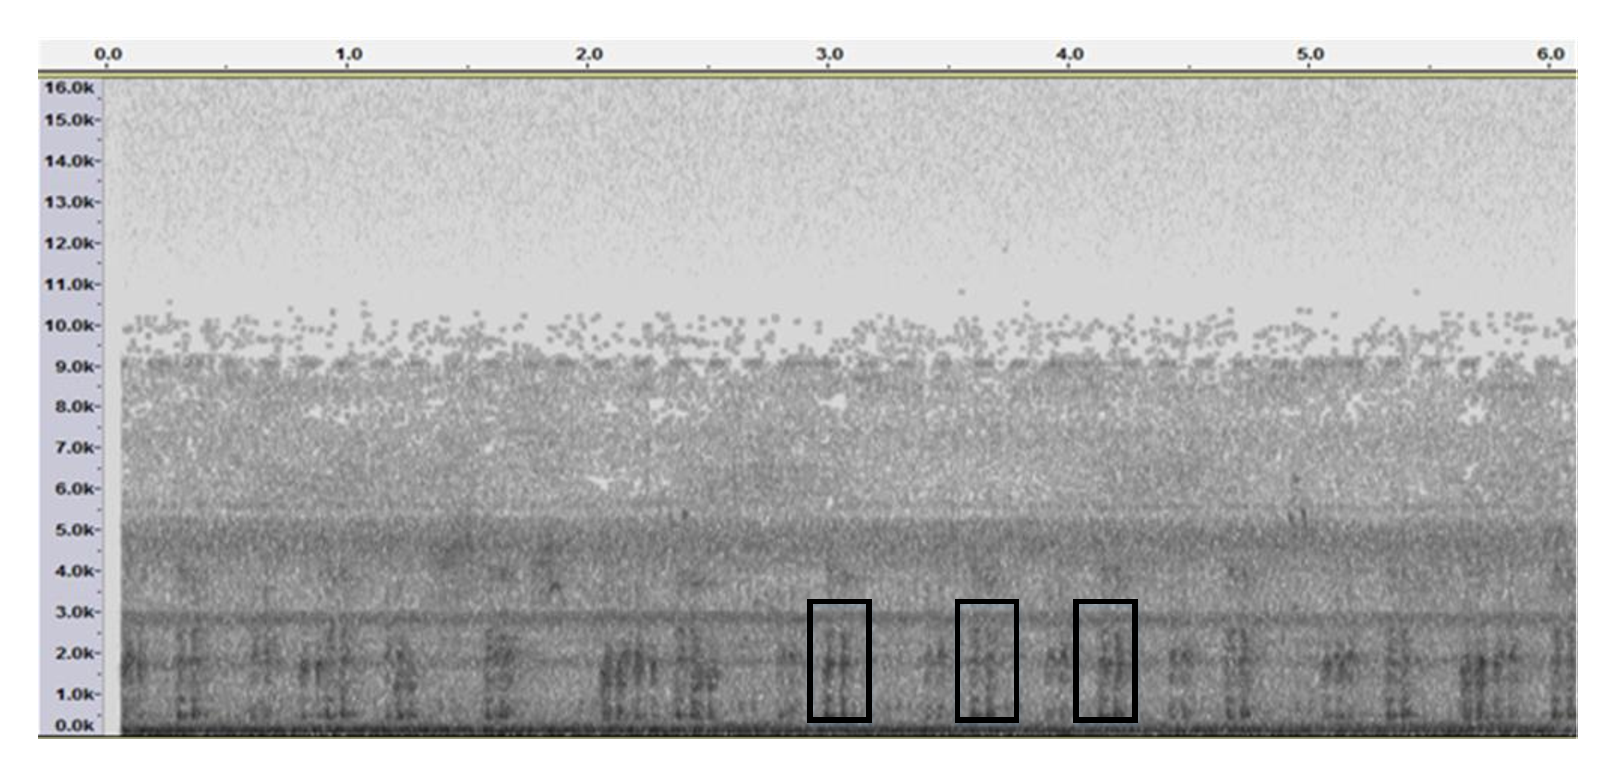
\includegraphics[width=\textwidth]{image/Ch1/spectrogram_mark.pdf}
\caption[Spectrogram of \textit{Litoria caerulea}]{Spectrogram of \textit{Litoria caerulea}, three syllable of \textit{Litoria caerulea} are annotated with one black rectangle, respectively.}
\label{fig:Ch1_spec_mark}
\end{figure}




One syllable is basically a sound that a frog produces with a single blow of air from the lungs \citep{huang2009frog}. For frog call classification, an elementary unit is one syllable. 
To get an intuitive sense of frog call structure, examples of different frog species in both waveform and spectrogram are shown in Table~\ref{tab:wav_spec_cd} and Table~\ref{tab:JCU_para}. For the waveform, x-axis and y-axis represent time and amplitude scales, respectively. The x-axis and y-axis of the spectrogram represent the time and frequency scales, respectively. The grey scale represents the acoustic intensity. 


%Six frog species, which are widely distributed in Queensland, Australia, are selected from David Stewart's CD to generate waveform and spectrogram \citep{CD}. For JCU recordings, eight frog species are selected. The parameters of those frog species are shown in Table \ref{tab:cd_parameter}.
%
%
%\begin{table}[htb!]
%\centering
%\caption[Averaged parameters of CD recordings]{Averaged parameters of ten syllables of six frog species (David Stewart's CD)}
%\label{tab:cd_parameter}
%\resizebox{\textwidth}{!}{
%\begin{tabular}{llll}\hline\hline
% \backslashbox{Frog \\ species}{Parameters}     & \begin{tabular}[c]{@{}l@{}}Syllable duration \\ (milliseconds)\end{tabular} & Dominant frequency (Hz) & \begin{tabular}[c]{@{}l@{}} Oscillation rate \\ (cycle/second) \end{tabular} \\\hline
%\textit{Bufo marinus}        &    NA   &   600 $\pm$ 30      &                                15 $\pm$ 5 \\
%\textit{Litoria caerulea}    &     500 $\pm$ 30                             &                        500 $\pm$ 75 &    50 $\pm$ 10                             \\
%\textit{Litoria fallax}      &        430 $\pm$ 25                          &                        4700 $\pm$ 450 &                70 $\pm$ 10                 \\
%\textit{Litoria gracillenta} &     430 $\pm$ 25                             &                        4700 $\pm$ 450 &                  70 $\pm$ 10               \\
%\textit{Litoria latopalmata} &       30 $\pm$ 5                           &                        1400 $\pm$ 120 &       5 $\pm$ 2                          \\
%\textit{Litoria rubella}     &   160 $\pm$ 15                               &                        4100 $\pm$ 380 &                            70 $\pm$ 10    \\\hline\hline
%\end{tabular}
%}
%\end{table}









\subsection{Acoustic event and background noise}
An acoustic event is a localised region of high intensity in a spectrogram. As we can see from Figure.~\ref{fig:label}, there are lots of acoustic events in an one-minute recording. This study focuses on the frog vocalisations, and frog calls are recorded as signals. Consequently, all the other events are called background noise. 
In this study, both high and low SNR recordings are investigated to build a robust frog call classification system. Most previous studies present the frog call classification system using high SNR recordings. The high SNR recordings often assume that there is only one frog species in each individual recording with few background noises ($SNR \geq 15 dB$). In contrast, most low SNR recordings consist of more than one frog species in an individual recording with lots of background noises ($SNR \leq 15 dB$). For the low SNR recordings, Table~\ref{tab:psd} show the power spectral density of signal and noise. It can be seen that the noise in low SNR recordings is often generated by several sources and broadband, which covers different frequency bands and leads to the frequency overlapping between the signal and noise. 
%Therefore, it is challenging to improve the classification performance in high SNR recordings over current frog call classification systems, and analyse the recordings containing background noise and simultaneous vocalising events.






\subsection{Frog call classification}

For a frog call classification system, it often consists of four parts (Figure.~\ref{fig:Ch1_flowchart}) : (1)signal pre-processing, which includes signal processing and noise reduction; (2) syllable segmentation, which is used to generate basic classification unit for frog calls; (3) feature extraction; (4) classification.  



\begin{figure}[htb!]
\centering
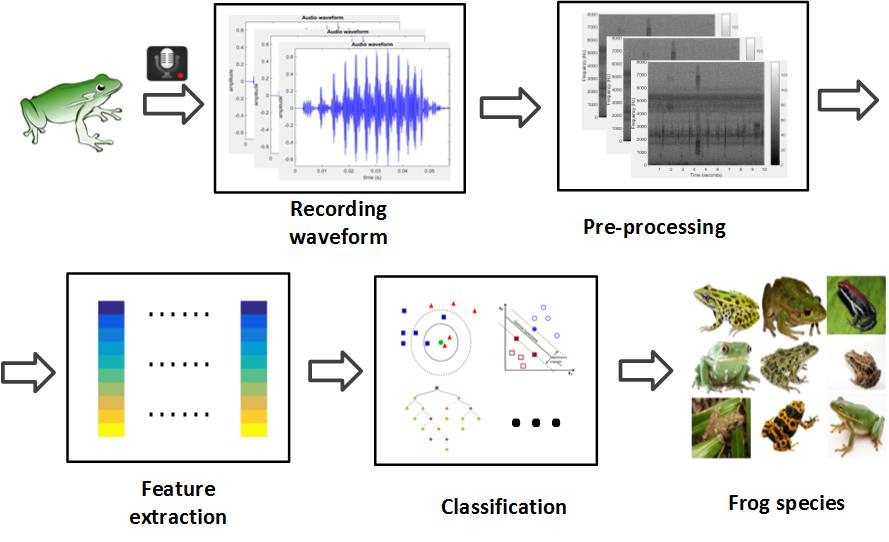
\includegraphics[width=\textwidth]{image/Ch1/flowchart.jpg}
\caption[Flowchart of a frog call classification system]{Flowchart of a frog call classification system}
\label{fig:Ch1_flowchart}
\end{figure}


\section{Research Challenges}
Most datasets used in previous frog call classification studies assume that there is only one frog species in each individual recordings. However, these resulting frog calls cannot reflect the characteristics of frog vocalisations in real-world situations, such as background noise, frog chorus, and other vocalising animals. To develop a robust frog call classification system for environmental recordings, two main challenges have been identified. 


\noindent \textbf{Challenge 1}: Most previous work studied frog call classification using high SNR recordings, the first challenge is thus to further improve the classification performance using high SNR recordings. Various acoustic features have been investigated for the classification of frog calls in high SNR recordings. Since our work finally aims to classify frog calls in low SNR recordings, most features that can successfully classify high SNR recordings cannot perform well for low SNR recordings. Consequently, it is still a big challenge to develop robust acoustic features to classify frog species in low SNR recordings. 

\noindent \textbf{Challenge 2}: Another challenge is the classification framework for studying frog vocalisations in low SNR recordings. Since most previous work assumed that each individual recording consists of only one frog species, a single-instance single-label (SISL) framework is suitable for classifying frog calls in those high SNR recordings. However, low SNR recordings often have different characteristics containing more than one frog species, the SISL framework is no longer suitable. Therefore, different classification frameworks need to be investigated to study frog vocalisations in low SNR recordings.


\section{Research questions}
The research questions are developed in order to solve the aforementioned challenges, which can be categorised into three parts. 

\begin{enumerate}
 \item How to improve the classification performance when addressing high SNR recordings?
 
\item How to develop robust acoustic features to classify frog calls in low SNR recordings?

\item How to employ suitable classification frameworks to classify multiple simultaneous vocalising frog species in low SNR recordings?
 
\end{enumerate}




\section{Aims and objectives}
This thesis aims to develop a robust frog call classification system to monitor the environment. For high SNR recordings, we want to improve the classification performance. As for the low SNR recordings, we plan to design novel frameworks to classify multiple simultaneously vocalising frog species. With our classification results, ecologists can then make decisions on how to protect and improve the health of frog populations. The specific research objectives are listed below.


\begin{enumerate}

\item	To improve the current representation schemes for modelling frog calls in high SNR recordings

\item 	To develop robust feature extraction methods for frog call classification in low SNR recordings 

\item   To investigate machine learning techniques (MIML learning and ML learning) to tackle the frog call classification problem in low SNR recordings

\end{enumerate}
 
 
 
\section{Significance and contributions}
For the development of sensor techniques, acoustic sensors have been widely deployed in the field for surveying vocalising animals. Different from recordings collected in the constrained environment, recordings collected in the field often have low SNR and consist of multiple simultaneous vocalising frog species. In this dissertation, we first investigate the high SNR recordings to further improve the classification performance of frog recordings with high SNR. 
Then, those features that can be used for studying frog calls in low SNR recordings are transplanted from high SNR recordings for further analysis.
Since field recordings often consists of multiple simultaneous vocalising frog species, both MIML and ML learning are used for the classification of those low SNR field recordings. Meanwhile, the frog calling activity can also be monitored based on the MIML and ML classification results.
With our developed frog call classification frameworks, ecologists can then analyse frogs by collecting audio data. It will significantly reduce the expert labour cost for monitoring frog calling activity of a particular area. The monitoring result can also help reveal the importance of environmental protection, which can be achieved via studying the correlation between the frog calling activity and weather variables. 

 
 
\section{Summary by chapters} 
 
This thesis is organised in the manner outlined in Figure.~\ref{fig:mainchapters}

\begin{figure}[htb!]
\centering
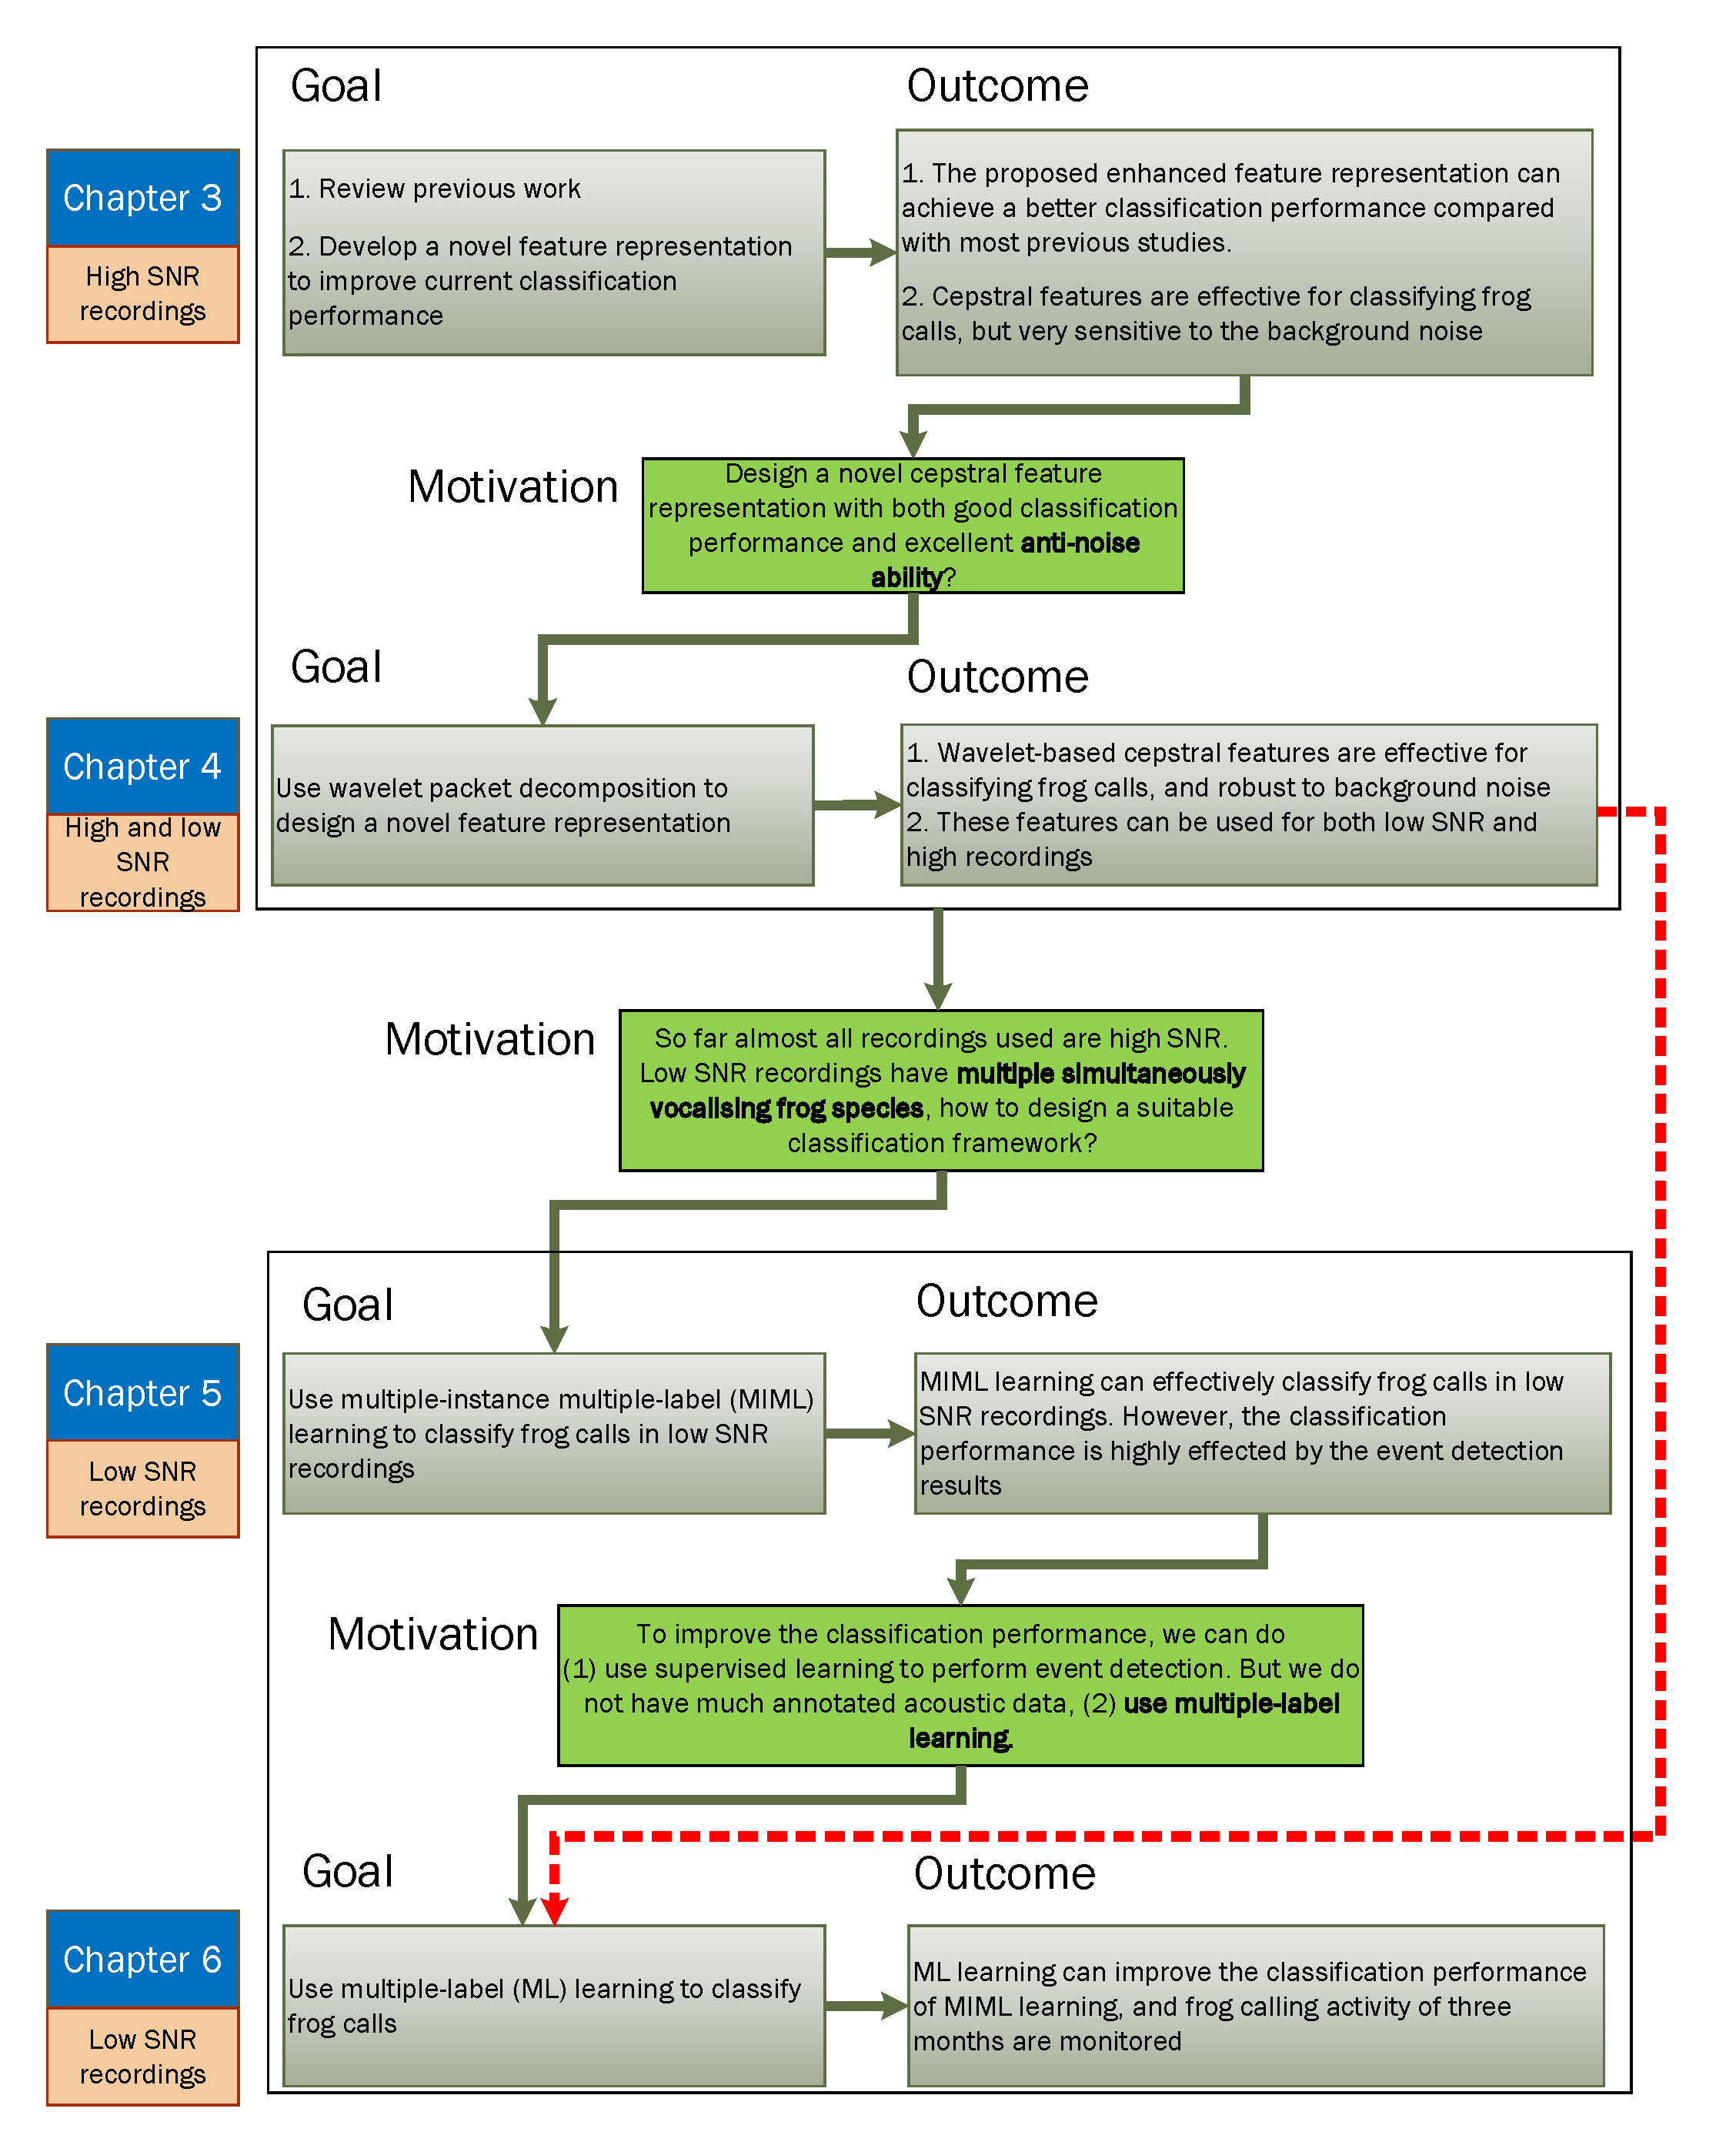
\includegraphics[width=\textwidth]{image/Ch1/structure_chapters.pdf}
\caption[Structure of the four main chapters of this thesis]{Structure of the four main chapters of this thesis}
\label{fig:mainchapters}
\end{figure}

Detailed description of each chapter is shown below:



\begin{itemize}
\item  Chapter \ref{cha:cha1Introduction} provides a brief introduction to the problem of "Acoustic classification of Australian frogs for ecosystem surveys". The motivation and background are first illustrated. Then specific to frog call classification, five basic concepts are presented to give a brief ideal about this research: environmental audio data, audio data analysis, frog call structure, acoustic event and background noise, and frog call classification system. Next, research problems and questions, aims and objectives, significance and contributions are proposed based on those five basic concepts. To be specific, there are three main objectives in this thesis. The remaining chapters are organised in the order of targeting those three objectives.

\item Chapter \ref{cha:cha2LiteratureReview} provide an overall literature review. The discussion separates the frog call classification system into signal pre-processing, feature extraction and classification. In addition, there are reviews for evaluation methods and previous experimental results. This chapter intends to provide the reader with a foundation for the research problem and necessary information about the state-of-the-art. Furthermore, the research gap in current literature is given, which provides a direction for the following work.


\item Chapter \ref{cha:cha4EnhancedFeature} presents an enhanced feature representation for frog call classification. An enhance feature representation is constructed via the combination of temporal, perceptual, and cepstral features. Five machine learning algorithms are evaluated with our proposed feature representation. This chapter aims to (1) review previous features used for frog call classification and build a best feature representation; (2) explore those previous features and study which can be adapted from high SNR recordings to low SNR recordings.


\item  Chapter \ref{cha:cha5Wavelet} discusses wavelet analysis for frog call classification. According to the conclusion from chapter \ref{cha:cha4EnhancedFeature}, we find that ceptral feature can achieve higher classification accuracy compared with temporal and perceptual features. But it is very sensitive to the background noise. Consequently, we design a novel cepstral feature representation with wavelet packet decomposition that have both high classification performance and a good anti-noise ability. It is because our research will move to low SNR recordings from high SNR recordings, rather than only focus on the low SNR recordings.


\item  Chapter \ref{cha:cha6MIML} discusses the use of multiple-instance multiple-label framework for frog call classification. To cope with low SNR recordings with multiple simultaneously vocalising frog species, the traditional single-instance single-label classification framework is no longer suitable. Therefore, we try to adopt other classification frameworks (such as MIML learning and ML learning). MIML learning is presented in this chapter. A MIML classification framework for studying is adopt to frogs. However, their syllables are detected using a supervised learning algorithm, which needs lots of annotated data. In our study, we are lack of those annotated frog recordings. A unsupervised learning method is developed to segment syllables, which is named \textit{acoustic event detection (AED)}. Then, three MIML learning classifiers are evaluated with extracted features from each syllables after applying a bagging algorithms. The classification performance is highly affected by the results of AED. Although our AED methods achieves a better results compared with previous AED methods, the results still need to be  further improved.


\item  Chapter \ref{cha:cha7ML} discusses the multiple-label learning for frog call classification. Since chapter \ref{cha:cha6MIML} shows that classification performance is highly affected by the AED results, and the AED results still need to be improved. This chapter uses ML learning to study low SNR recordings with multiple simultaneously vocalising frog species, where AED is not necessary for the classification. In contrast, AED is used to predict the frog abundance. The cepstral feature representation proposed in chapter \ref{cha:cha5Wavelet} is used, where a simple but effective method is used to modify it. Both the results of AED and ML classification are applied to recordings over three months. 



\item  Chapter \ref{cha:cha8Conclusions} summarises and concludes the thesis, claims the achievements, and recommends possible directions in future work.



\end{itemize}





